\section{Design Space}
\label{sec:dspace}

The narrow interface exposed by storage systems has been a boon in allowing
systems and applications to evolve independently, in effect limiting the size
of the design space where applications couple with storage. Programmable
storage lifts the veil on the system, and with it, forces developers of higher-level services
to confront a large and expanding set of possible designs.

In this section we elucidate the matter of design space size and complexity in
programmable storage. We report on our experience building and optimizing
\emph{multiple} functionally equivalent implementations of the CORFU protocol
in Ceph, demonstrating that static selection of optimization strategies and tuning
decisions can lead to performance portability challenges in programmable
storage sytems.

\subsection{System Tunables and Hardware}

A recent version of Ceph (v10.2.0-1281-g1f03205) has 994 tunables parameters,
where 195 of them pertain to the object server itself and 95 of them focus on
low-level storage abstractions built on XFS or BlueStore.  Ceph also has
tunables for the subsystems it uses, like LevelDB (10 tunables), RocksDB (5
tunables), its own key-value stores (5 tunables), its object cache (6
tunables), its journals (24 tunables), and its other optional object stores
like BlueStore (49 tunables).  Auto-tuning~\cite{behzad:sc2013-autotuning}
techniques have been applied to systems with a large space of parameters with
limited success, but the challenge is exacerbated in the context of
application-specific modifications and workloads that change dynamically.

{\bf Hardware.} Ceph is designed to run on a wide variety of commodity
hardware as well as new NVMe devices. All these devices have their own set of
characteristics and tunables (e.g., the IO operation scheduler type). In our
experiments, we tested SSD, HDDs, NVMe devices and discovered a wide range of
behaviors and performance profiles. While we generally observe the expected
result of faster devices resulting in better application performance, choosing
the best implementation strategy is highly dependent on hardware. The changes
in Ceph required to fully exploit the performance profile of NVMe, persistent
memory, and RDMA networks will likely result in new design trade-offs for
application-specific interface designs.

\textbf{Takeaway:} Evolving hardware and system tunables present a challenge
in optimizing systems, even in static cases with fixed workloads. Programmable
storage approaches that introduce application-specific interfaces that are
sensitive to changes in workloads and the cost models of low-level interfaces
that are subject to change  greatly increase the design space and set of
concerns to be addressed by programmers.

\subsection{Software}

The primary source of complexity in large storage systems is unsurprisingly
the vast amount of software written to handle challenges like fault-tolerance
and consistency in distributed heterogeneous environments. We have found that
even routine upgrades can cause performance regressions that introduce
challenges for adopters of a programmable storage approach to development.

The CORFU protocol stripes a log across a cluster of storage
devices that each expose a custom 64-bit write-once address space for reading
and writing log entries. While this interface can be built directly into flash
devices~\cite{wei:systor13}, we constructed four different versions in Ceph
each as a software abstraction over the existing object interface.
Each of our software-based implementations differ in their optimization
strategy of utilizing internal system interfaces. For instance one
implementation uses a key-value interface to manage the address space index
and entry data, while another implementation stores the entry data using a
byte-addressable interface. 

Figure~\ref{fig:phy-design} shows the append throughput of four such
implementations run on two versions of Ceph from 2014 and 2016. The first
observation to be made is that performance in general is significantly better
in the newer version of Ceph. However, what is interesting is the relationship
between the implementations. Run on a version of Ceph from 2014, the top two
implementations perform with nearly identical throughput, but have strikingly
different implementation complexities. The performance of the same
implementations on a newer version of Ceph illustrate a challenge: given a
reasonable choice of a simpler implementation in 2014, a storage interface
will perform worse in 2016, requiring significant rework of low-level
interface implementations.

\begin{figure*}[t]
    \centering
    \begin{subfigure}[b]{.33\linewidth}
        \centering
        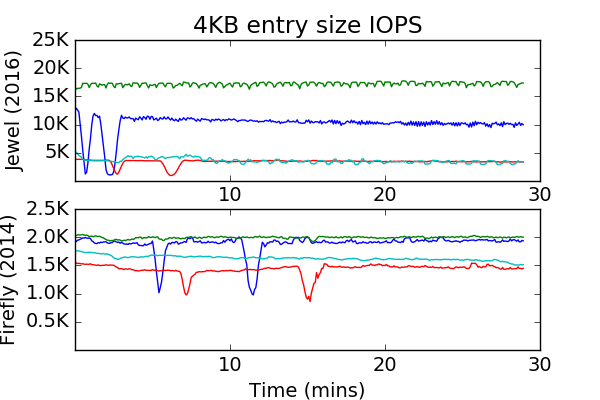
\includegraphics[width=1.0\linewidth]{jewel_v_firefly_pd.png}
        \caption{}
        %\caption{Relative performance differences can be drastic after a software
        %upgrade of the underlying storage system.}
        \label{fig:phy-design}
    \end{subfigure}
    \begin{subfigure}[b]{.33\linewidth}
        \centering
        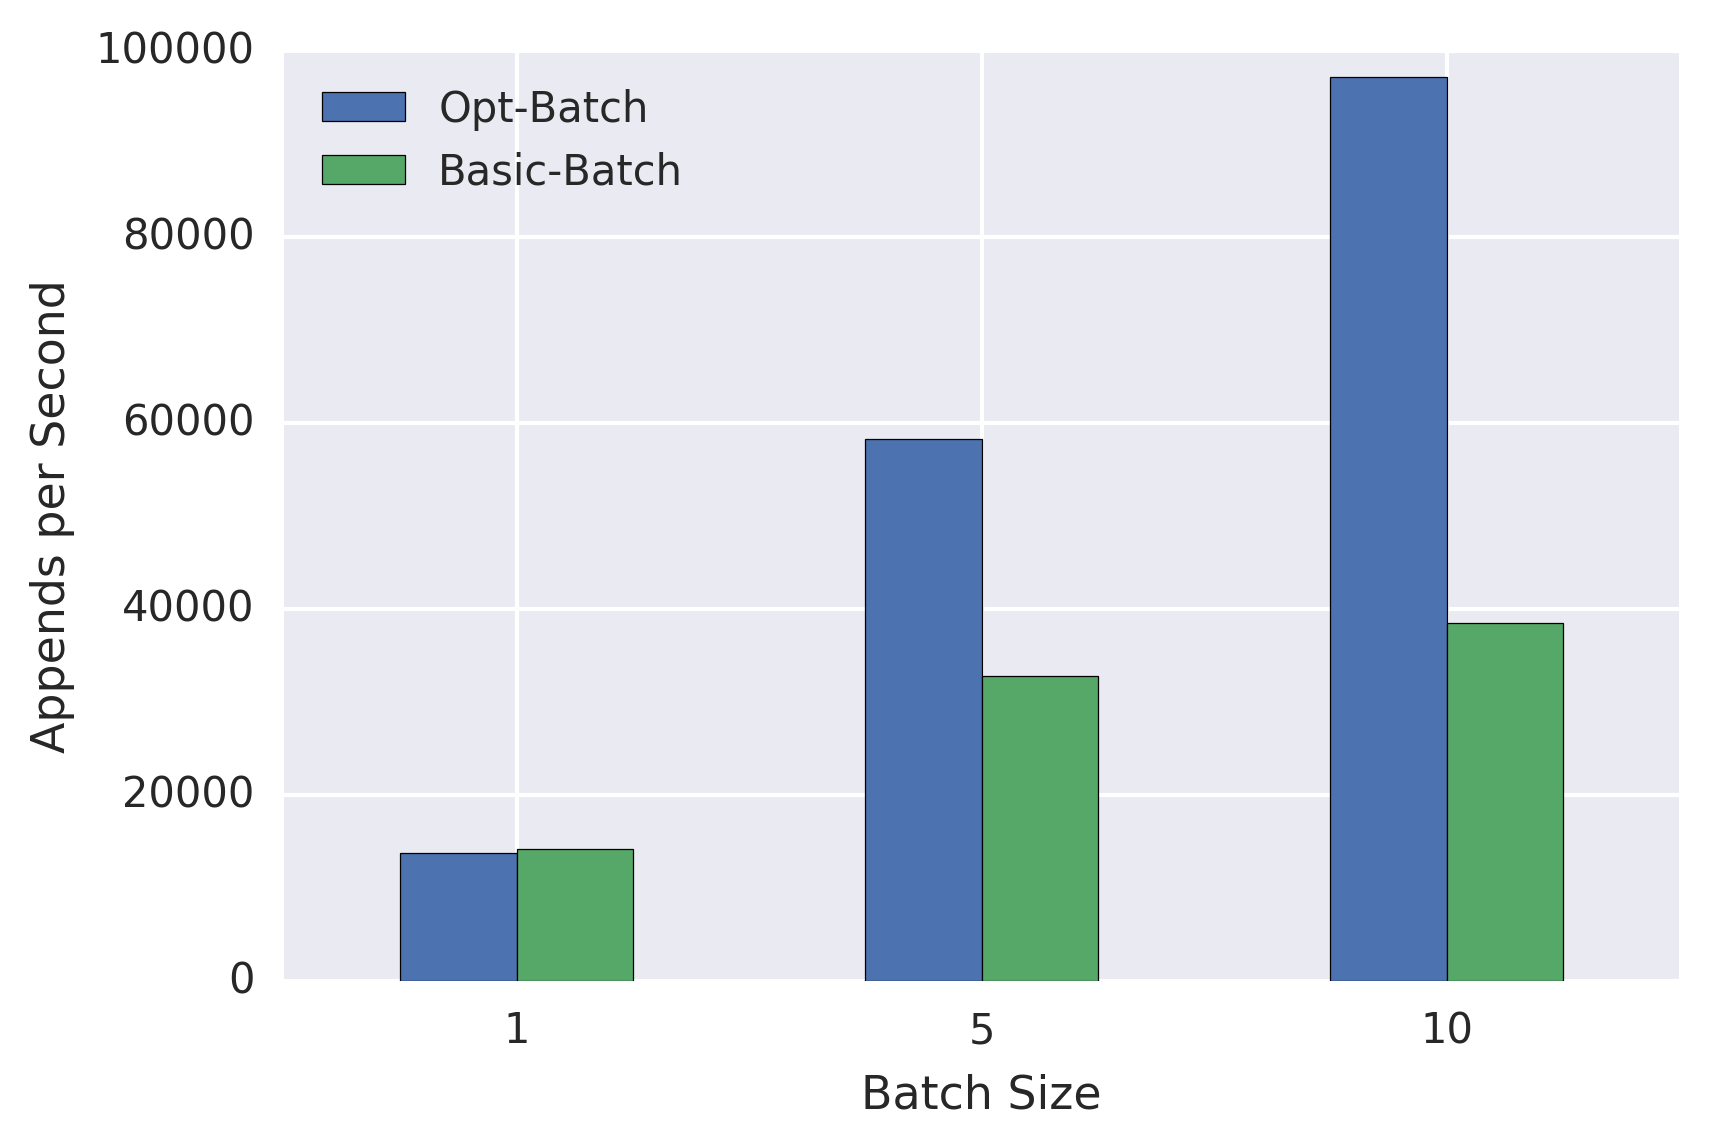
\includegraphics[width=1.0\linewidth]{batching.png}
        \caption{}
        %\caption{Total throughput with and without batching.}
        \label{fig:batching}
    \end{subfigure}
    \begin{subfigure}[b]{.33\linewidth}
        \centering
        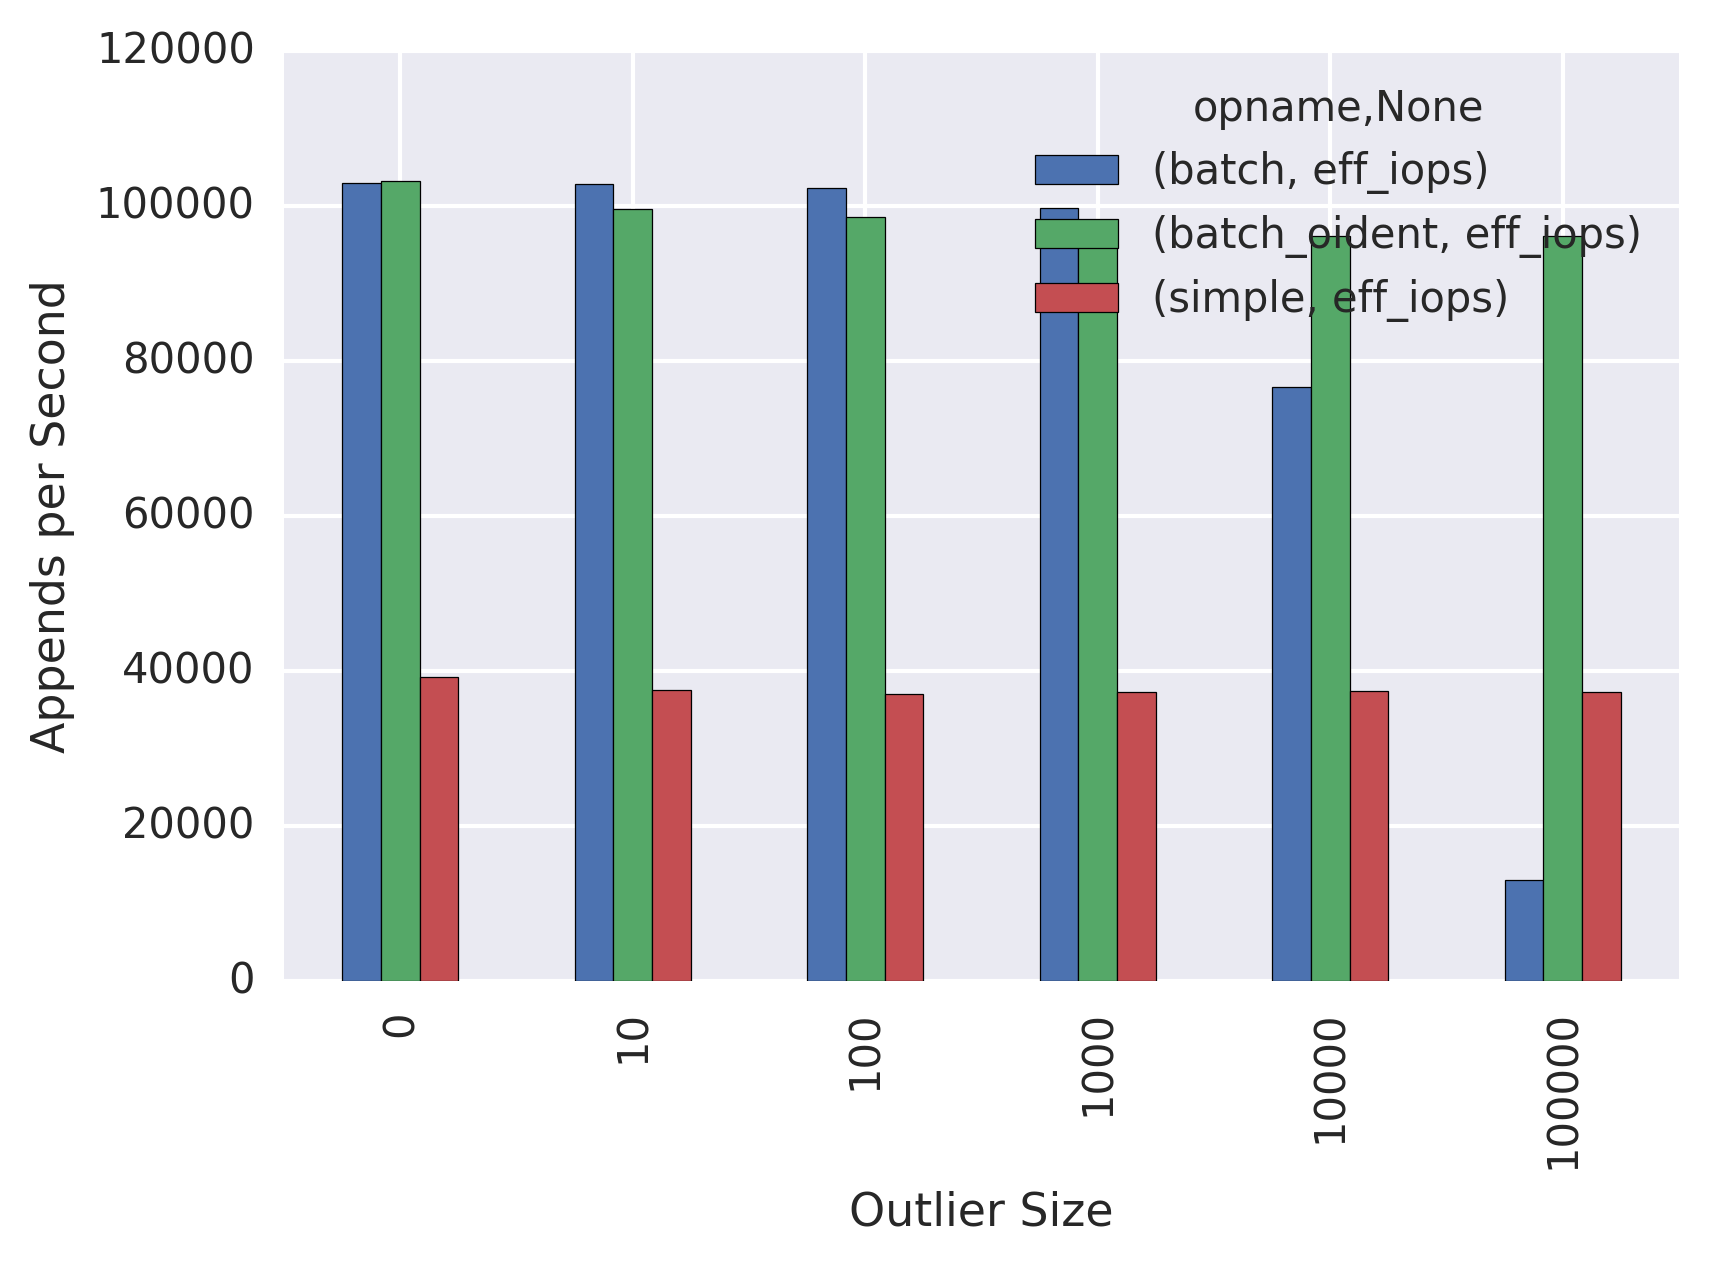
\includegraphics[width=1.0\linewidth]{batching-outlier-detect.png}
        \caption{}
        %\caption{Identifying and handling an outlier independently maintains the
        %beneifts of batching without the performance degredation of unecessarily
        %large I/O requests.}
        \label{fig:batching-outlier}
    \end{subfigure}
    \caption{(a) relative performance differences can be drastic after storage
    software upgrade. (b) total throughput with and without batching.  (c)
    identifying and handling an outlier independently maintains the benefits
    of batching without the performance degradation of unnecessarily large I/O
    requests.}
\end{figure*}

\subsubsection{Application-specific Group Commit}

Group commit is a technique used in database query execution that combines
multiple transactions in order to amortize over per-transaction fixed costs
like logging. Figure~\ref{fig:batching} shows the performance impact of using
a \emph{group commit}-like technique for batching log appends from independent
clients into a single request.  The \emph{Basic-Batch} case implements group
commit at the request level, but processes each sub-request (i.e.  append)
independently using low-level I/O interfaces. The modest performance increase
is attributed to a reduction in average per-request costs related to network
round-trips. Compared with the \emph{Basic-Batch} case, the \emph{Opt-Batch}
implementation is able to achieve significantly higher performance by
constructing more efficient I/O requests using range queries and data sieving
techniques~\cite{x} afforded by the low-level I/O interfaces.

The batched execution technique of group commit can significantly increase
throughput, but the story is much more complex. The ability to apply this
technique requires tuning parameters such as adding artificial delays to
increase batch size that will also affect other metrics such as latency.
While the performance impact of application-specific batching is significant,
techniques such as range queries and data sieving are sensitive to outliers
that can occur with buggy or slow clients.

When outliers occur in a batch, naively building large I/O requests can result
in a large amount of wasted I/O.  Figure~\ref{fig:batching-outlier} highlights
this scope of this challenge. The \emph{Basic-Batch} case handles each request
in a batch independently, and while it performs relatively worse than the
other techniques, it is not sensitive to outliers. The \emph{Opt-Batch}
implementation achieves high append throughput, but performance degrades as
the magnitude of the outlier in the batch increases. In contrast, an
\emph{Outlier-Aware} policy applies a simple heuristic to identify outliers
and handle them independently, resulting in only a slight decrease in
performance over the best case.

\textbf{Takeaway:} Choosing the best implementation of a storage interface
depends on the timing of development (Ceph version), the expertise of
programmers and administrators (Ceph features), the tuning parameters and hardware
selection, as well as system-level and application-specific workload changes.
A direct consequence of such a large design space is that engineers are forced
to duplicate efforts when hardware and software characteristics change. This
is bad: it's unnecessary on-going work, and increases the risk of introducing
bugs that in the best case affect a single application, and in monolithic
designs are more likely to cause systemic data loss.

We believe that with a better understanding of application and interface
semantics there are better approaches than hard-coded and hand-tuned
implementations.  An ideal solution to these challenges is an automated system
search of \emph{implementations}---not simply tuning parameters---based on
programmer produced specifications of storage interfaces in a way that is
independent of optimization strategies, and guaranteed to not introduce
correctness bugs. Next we'll discuss a candidate approach using a declarative
language for interface specification.
